\begin{figure}[h]
	\centering
	\setlength{\imgWidth}{1.55in}
	\addtolength{\tabcolsep}{-3.5pt}
	\begin{tabular}{cccc}
		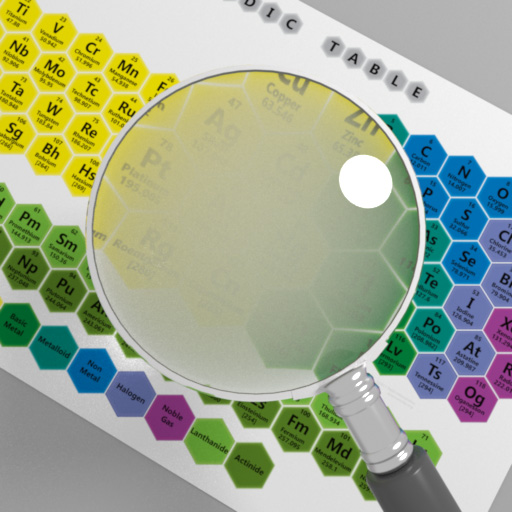
\includegraphics[width=\imgWidth]{layeredbsdf/results/magnify_g9.jpg} &
		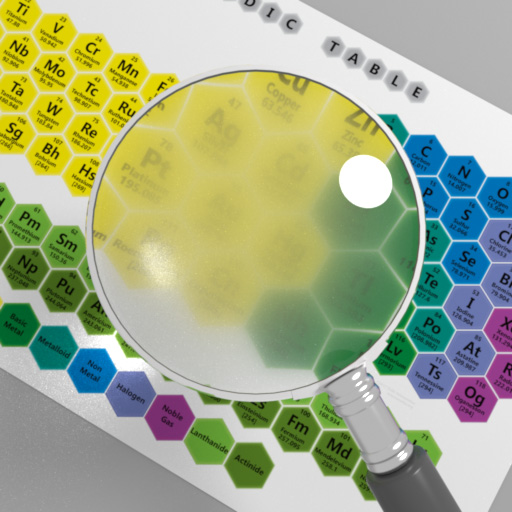
\includegraphics[width=\imgWidth]{layeredbsdf/results/magnify_g99.jpg} &
		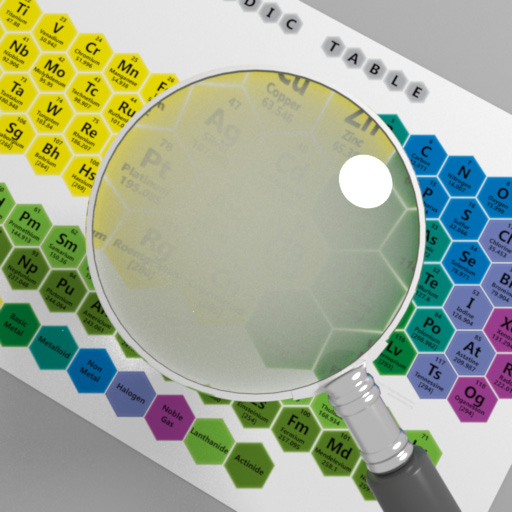
\includegraphics[width=\imgWidth]{layeredbsdf/results/magnify_vmf10.jpg} &
		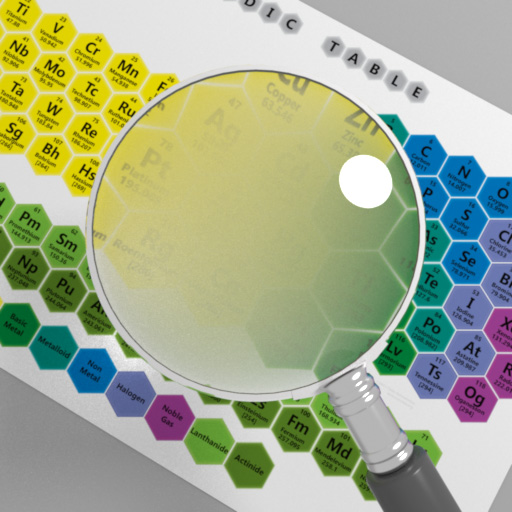
\includegraphics[width=\imgWidth]{layeredbsdf/results/magnify_vmf100.jpg}\\
		HG ($g = 0.9$) & HG ($g = 0.99$) & vMF ($\kappa = 10$) & vMF ($\kappa = 100$)
	\end{tabular}
	\caption[Reflection and transmission B]{\label{fig:layeredbsdf:magnifier}
		\textbf{Reflection and transmission:}
		A flat surface with a layered BSDF of spatially varying thickness (which captures the shape of real convex lens). A range of spatially varying and physically plausible blurring effects can be achieved by varying phase functions.
	}
\end{figure}